\ifx\allfiles\undefined
\documentclass{article}
\usepackage{graphicx}
\usepackage{geometry}
\usepackage{hyperref}
\usepackage{amssymb}
\usepackage{booktabs}
\usepackage{tabularx}
\usepackage{amsthm}
\usepackage{amsmath}
\usepackage{enumitem}
\usepackage{tikz}
\usetikzlibrary{automata, positioning, arrows}

\geometry{left=1.2in, right=1.2in, top=1.5in, bottom=1.5in}
\linespread{1.5}%行距

% 设置列表环境的上下间距
\setenumerate[1]{itemsep=5pt,partopsep=0pt,parsep=\parskip,topsep=5pt}
\setitemize[1]{itemsep=5pt,partopsep=0pt,parsep=\parskip,topsep=5pt}
\setdescription{itemsep=5pt,partopsep=0pt,parsep=\parskip,topsep=5pt}

\theoremstyle{definition}
\newtheorem{defn}{\textbf{\textit{def}}}[section]
\newtheorem{prop}{\textbf{\textit{prop}}}[section]
\newtheorem{thm}[defn]{\textbf{\textit{thm}}}

\newtheorem{lemma}{lemma}[section]% 引理 推论 准则 共用一个编号计数
\newtheorem{corollary}[lemma]{\textbf{\textit{corollary}}}
\newtheorem{criterion}[lemma]{\textbf{\textit{criterion}}}

\newtheorem{proposition}{\textbf{\textit{proposition}}}[section]
\newtheorem{example}{\textbf{\textit{e.g.}}}[section]
\newtheorem{exercises}{\textbf{\textit{exercises}}}[section]
\newtheorem*{remark}{\textbf{\textit{remark}}}

\newenvironment{solution}{\par{\textit{solution}}\;}{\qed\par}

\def\R{\mathbb{R}} % 实数域
\def\N{\mathbb{N}} % 自然数域
\def\Q{\mathbb{Q}} % 有理数域
\def\eps{\varepsilon} %ε

\graphicspath{ {pictures/},{../pictures/}}  % 配置图形文件检索目录
\begin{document}
\setcounter{section}{2}
\else
\fi
\section{Algorithm and Turing Machines}

\subsection{Turing machines}

\textit{An algorithm is a mechanical process to be followed in calculations or other problem-solving operation.}

\begin{example}
    \

    \begin{enumerate}
        \item \textit{addition,substraction,multiplication,division}
        \item \textit{\textbf{Euclidean algorithm} for gcd:}
        $gcd(210,25)=gcd(45,30)=gcd(30,15)=gcd(15,0)$
        \item \textit{selection quicksort}
        \item \textit{Dijkstra's algorithm for shortest path}
    \end{enumerate}
\end{example}

\textit{\\In 1936 for the first time, Alan Turing rigorously defined algorithms}

\begin{figure}[H]
    \begin{center}
        \includegraphics[scale = 0.5]{3.1.png}
    \end{center}
    \caption{\textit{Schematic of a Turing machine}}
\end{figure}

\begin{enumerate}
    \item \textit{It uses an infinite tape as its unlimited memory}
    \item \textit{It has a tape head that can read and write symbols and move around on the tape}  
\end{enumerate}

\begin{defn}
    \textit{(Turing Machine)}

    \textit{A \textbf{Turing machine} is a 7-tuple, $(Q, \Sigma, \Gamma , \delta, q_0, \underbrace{q_{accept}, q_{reject}}_{q_{end}})$, where:}

    \begin{enumerate}
        \item \textit{Q is a set of states}
        \item \textit{$\Sigma$ is the input alphabet not containing the blank symbol $\sqcup $}
        \item \textit{$\Gamma$ is the tape alphabet, where $\sqcup\in \Gamma$ and $\Sigma\subseteq\Gamma$}
        \item \textit{$\delta:Q\times\Gamma\rightarrow Q\time\Gamma\times\{L,R\}$ is the transive function}
        \item \textit{$q_0\in Q$ is the start state}
        \item \textit{$q_{accept}\in Q$ is the accept state}
        \item \textit{$q_{reject}\in Q$ is the reject state, where $q_{accept}\neq q_{reject}$}
    \end{enumerate}
\end{defn}

\begin{example}
    \

    \begin{enumerate}
        \item \textit{Input a binary number n (least significant bit first), output n+1}

        \textit{Input: $101\sqcup\sqcup$ \\ Output: $011\sqcup\sqcup$}
    

        \begin{remark}
            \textit{this is a computation problem(6-tuple)}
        \end{remark}

        \bgpic
            \node[state,initial] (A) {$q_0$};
            \node[state,accepting] [right = 4cm of A] (B) {$q_{end}$};

            \path (A) edge [loop below] node {$1\rightarrow0,R$} (A)
                    edge              node {$0\rightarrow1,S$ \ \ \ \ $\sqcup\rightarrow1,S$} (B);
        \end{tikzpicture}

        \item \textit{decide if $w\in\{0,1\}^*$ is a palindrome, i.e. $w = w^R$}

        \item \textit{decide $L = \{0^{2^n},n\geq0\}$, where $\Sigma = \{0\}$}
        
        \textit{\textbf{IDEA}}

        \begin{enumerate}
            \item \textit{If there is a single 0, accept it}
            \item \textit{Sweep left to right across the tape, crossing off every other 0.}
            \item \textit{If the tape contained more than a single 0 and the
            number of 0s was odd, reject}
            \item \textit{Return the head to the left-hand end of the tape}
            \item \textit{go to step1}
        \end{enumerate}

        \begin{figure}[H]
            \begin{center}
                \includegraphics[scale = 0.4]{3.2.png}
            \end{center}
            \caption{\textit{State diagram for Turing machine M2}}
        \end{figure}

        \item \textit{$L = \{w\#w,w\in\{0,1\}^*\}$}

        \begin{figure}[H]
            \begin{center}
                \includegraphics[scale = 0.4]{3.3.png}
            \end{center}
            \caption{\textit{State diagram for Turing machine M1}}
        \end{figure}
    \end{enumerate}
\end{example}

\begin{exercises}
    \

    \begin{enumerate}
        \item \textit{Binary comparison. $L = \{x,y|x,y\in\{0,1\}^*x\geq y,$ most significantbit first, no leading 0 unless the number is 0\}}
        \item \textit{Binary add 1}
        \item \textit{L = \{$0^n1^n$\}}
    \end{enumerate}
\end{exercises}

\begin{defn}
    \textit{Let $L\subset \{0,1\}^*$, M be a Turing Machine. Say M decides L in time T(n) if for $\forall x \in \{0,1\}^*$:}

    \begin{enumerate}
        \item \textit{M halts in T(n) steps}
        \item \textit{If $x\in L$, then M accepts x}
        \item \textit{If $x\notin L$, then M rejects x}
    \end{enumerate}
\end{defn}

\begin{defn}
    \textit{Let $L\subseteq \{0,1\}^*$. Call L(Turing Machine) decidable if there is a Turing Machine decides it}
\end{defn}

\begin{remark}
    \textit{On an input x, a TM may accept, reject, or loop forever}

    \textit{In \textbf{definition 3.2}, the machine should never loop forever}
\end{remark}

\begin{defn}
    \textit{Let M be a TM, the set of strings that M accepts is the language recognized by M, denoted by L(M)}
\end{defn}

\begin{defn}
    \textit{Let $L\subseteq \{0,1\}^*.$ Call L(Turing) recognizable if there is some TM recognizes it}
\end{defn}

\begin{remark}
    \textit{Obviously, every decidable language is recognizable. While the converse is not true, e.g. $L = \{<M,x>$,M halts on x\}}
\end{remark}

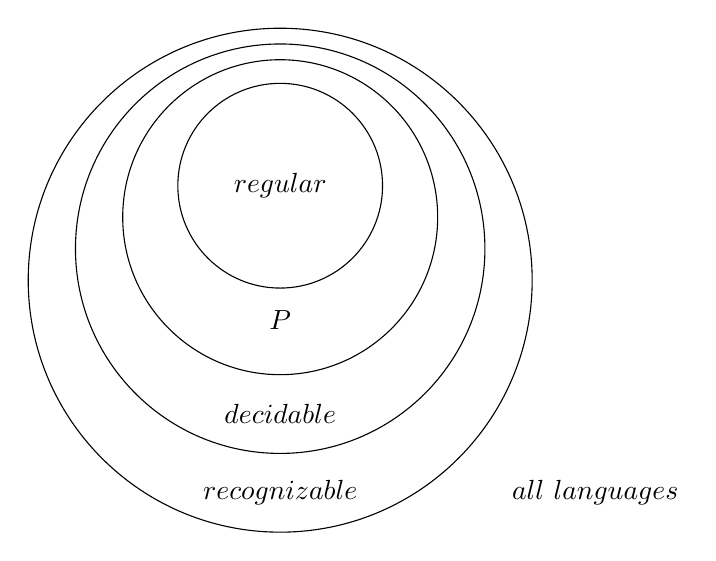
\begin{tikzpicture}
    \draw (0,1.5) circle (3.2cm);
    \draw (0,1.9) circle (2.6cm);
    \draw (0,2.3) circle (2cm);
    \draw (0,2.7) circle (1.3cm);
    

    % Add text
    \node at (0,2.7) {$regular$};
    \node at (0,1) {$P$};
    \node at (0,-0.2) {$decidable$};
    \node at (0,-1.2) {$recognizable$};
    \node at (4,-1.2) {$all~languages$};
\end{tikzpicture}

\begin{defn}
    \textit{Let $f:\{0,1\}^*\rightarrow \{0,1\}^*\cup\{undefined\}$. Say TM M computes f in time T(n) if for $\forall x\in \{0,1\}^*$, with $f(x)\neq undefined$, M halts with f(x) on its tape in at most $T(|x|)$ steps}
\end{defn}

\textit{\\What is algorithm? An algorithm is A Turing Machine. Despite its simplicity, it is capable of implementing any computer algorithm.\\ "Everything should be made as simple as possible, but no simpler."}

\subsection{Variants of Turing Machines}

\begin{lemma}
    \textit{If language $L\subseteq \{0,1\}^*$ is decidable in time T(n) by a Turing Machine on alphabet $\varGamma$, then it is decidable in time $O(log|\varGamma| T(n)) = O_\varGamma(T(n))$ by a Turing Machine on alphabet $\varGamma = \{0,1,\sqcup,\vartriangleright  \}$}

    \begin{proof}
        \textit{Encode any symbol in $\varGamma$ using $k = \lceil log_2|\varGamma|\rceil = O(log|\varGamma|)$ bits. To simulate one step of M, the new Turing Machine will:}

        \begin{enumerate}
            \item \textit{use k steps to read a symbol $a\in \varGamma$}
            \item \textit{transit to next step q', and get the new symbol b(to overwrite a)}
            \item \textit{overwrite a by b}
            \item \textit{go left or right for k steps, or stay}
        \end{enumerate}

        \textit{In total, the simulation (for one step) takes less than k+1+k+k = O(k)}
    \end{proof}
\end{lemma}

\begin{defn}
    \textit{A k-tape Turing Machine M is a 7-tuple $(Q,\Sigma,\varGamma,\delta,q_0,q_{accept},q_{reject})$, where:}
    
    $\delta:Q\times\varGamma^k\rightarrow Q\times\varGamma^k\times\{L,R,S\}^k$

    \textit{Usually, the first tape is the input tape, the last tape is the output tape, and the remaining tapes are work tapes.}

    \textit{A multiple Turing Machine is an O(1)-tape Turing Machine.}

    \begin{figure}[H]
        \begin{center}
            \includegraphics[scale = 0.6]{3.4.png}
        \end{center}
        \caption{\textit{3-tape Turing Machine}}
    \end{figure}
\end{defn}

\begin{lemma}
    \textit{Let $L\subseteq \Sigma^*$, If L is decidable by a k-tape Turing Machine in time T(n), then it is decidable by a single-tape Turing Machine in time $O(kT(n)^2) \textcolor{red}{\neq O(T(n)^2)}$}

    \begin{proof}
        \textit{Use location $i-1,k+i-1,2k+i-1,...$ to store the contents of the $i^{th}$ tape, where $i = 1,2,...,k$. For $\forall a\in\varGamma$, introduce $a,\widehat{a} \in \varGamma$, where $\widehat{a}$ denotes the location of the head.}

        \textit{To simulate one step of M, single-tape Turing Machine M' will:}

        \begin{enumerate}
            \item \textit{sweep the tape from left to right to read k symbols marked by $\widehat{~}$}
            \item \textit{apply M's transition function $\delta$ to determine the next state}
            \item \textit{sweep back from right to left to update k symbols, if needed, and move $\widehat{}$ if needed}
        \end{enumerate}

        \textit{In total, 1.2.3. take T(n)+1+O(kT(n)) = O(kT(n))}
    \end{proof}
\end{lemma}

\newpage

\begin{figure}[H]
    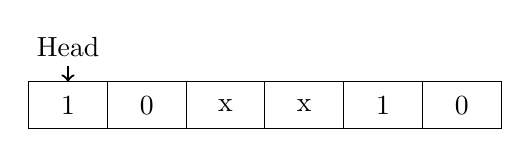
\begin{tikzpicture}
        \def\n{6} % 定义磁带上的格子数量
        \def\cellwidth{1} % 格子宽度
        \def\cellheight{0.6} % 格子高度
      
        % 绘制磁带
        \draw (0,0) rectangle (\n*\cellwidth, \cellheight);
        \foreach \i in {1,...,\n} {
          \draw (\i*\cellwidth,0) -- (\i*\cellwidth,\cellheight);
        }
      
        % 在格子上添加内容
        \foreach \i/\content in {1/1, 2/0, 3/x, 4/x, 5/1, 6/0} {
          \node at (\i*\cellwidth-\cellwidth/2, \cellheight/2) {\content};
        }
      
        % 标记当前头部位置
        \node[above] at (\cellwidth/2, \cellheight+0.2) {Head};
        \draw[->,thick] (\cellwidth/2,\cellheight+0.2) -- (\cellwidth/2,\cellheight);
      \end{tikzpicture}
    
      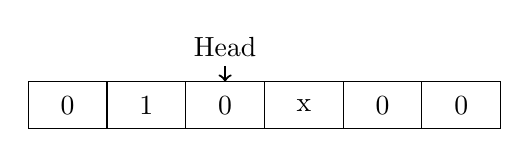
\begin{tikzpicture}
        \def\n{6}
        \def\cellwidth{1}
        \def\cellheight{0.6}
      
        \draw (0,0) rectangle (\n*\cellwidth, \cellheight);
        \foreach \i in {1,...,\n} {
          \draw (\i*\cellwidth,0) -- (\i*\cellwidth,\cellheight);
        }
    
        \foreach \i/\content in {1/0, 2/1, 3/0, 4/x, 5/0, 6/0} {
          \node at (\i*\cellwidth-\cellwidth/2, \cellheight/2) {\content};
        }
    
        \node[above] at (\cellwidth*2.5, \cellheight+0.2) {Head};
        \draw[->,thick] (\cellwidth*2.5,\cellheight+0.2) -- (\cellwidth*2.5,\cellheight);
      \end{tikzpicture}
    
    \caption{A two tape Turing Machine}
\end{figure}


\begin{figure}[H]

      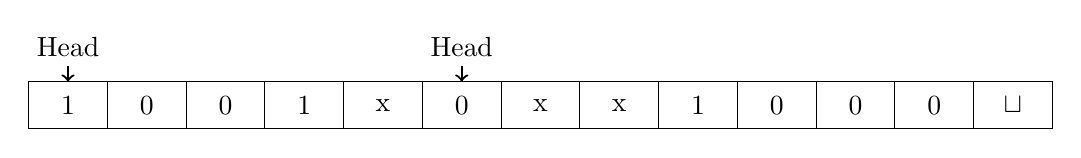
\begin{tikzpicture}
        \def\n{13}
        \def\cellwidth{1}
        \def\cellheight{0.6}
      
        \draw (0,0) rectangle (\n*\cellwidth, \cellheight);
        \foreach \i in {1,...,\n} {
          \draw (\i*\cellwidth,0) -- (\i*\cellwidth,\cellheight);
        }
      
        \foreach \i/\content in {1/1, 2/0, 3/0, 4/1, 5/x, 6/0, 7/x, 8/x, 9/1, 10/0, 11/0, 12/0, 13/$\sqcup$} {
          \node at (\i*\cellwidth-\cellwidth/2, \cellheight/2) {\content};
        }
      
        \node[above] at (\cellwidth/2, \cellheight+0.2) {Head};
        \draw[->,thick] (\cellwidth/2,\cellheight+0.2) -- (\cellwidth/2,\cellheight);
        \node[above] at (\cellwidth*5.5, \cellheight+0.2) {Head};
        \draw[->,thick] (\cellwidth*5.5,\cellheight+0.2) -- (\cellwidth*5.5,\cellheight);
    
      \end{tikzpicture}

      \caption{Representing two tapes with one}
\end{figure}

\textit{\\A \textbf{Bidirectional-tape Turing Machine} is a Turing Machine whose tape is infinite in both directions}

\begin{figure}[H]
    \begin{center}
        \includegraphics[scale = 0.5]{3.5.png}
    \end{center}

    \caption{\textit{A bidirectional-tape Turing Machine}}
\end{figure}

\begin{lemma}
    \textit{Let $L\subseteq \Sigma^*$. If L is decidable by a bidirectional-tape Turing Machine in T(n), then it is decidable by a single-tape Turing Machine in O(T(n)) time.}
    \begin{proof}
        \textit{Index the biderectional tape by $\Z$, map location i to}

        \[  
            \begin{cases}
                2i , i\geq0 \\
                -2i - 1 , i < 0 \\
            \end{cases}
        \]

        \newpage

        \textit{For every step of M, M' will}

        \begin{enumerate}
            \item \textit{read the symbol}
            \item \textit{transit to the next state}
            \item \textit{update the symbol}
            \item \textit{move left or right for two steps, if needed}
        \end{enumerate}

        \textit{It takes O(1) to simulate one step. In total, the running time is O(T(n))}
    \end{proof}
\end{lemma}

\begin{defn}
    \textit{Random access memory(RAM) Turing machine is a TM with random access memory:}

    \begin{enumerate}
        \item \textit{M has an infinite memory tape A indexed by N}
        \item \textit{One of M's tapes is the address tape}
        \item \textit{$\varGamma$ contains two speed symbols R(read) and W(write)}
        \item \textit{Q has some special states $Q_{access}\subseteq Q$\\Whenever M gets into a state $q\in Q_{access}$}
        \begin{enumerate}
            \item \textit{If the address tape contains iR, the value $A[i]$ is written to the cell next to R}
            \item \textit{If the address tape contains $iW\sigma$, then set $A[i]$ to symbol $\sigma$}
        \end{enumerate}
    \end{enumerate}

    \textit{Assume the TAM Turing Machine M has k work tapes and an address.}
    
    \textit{Then $M = (Q,\Sigma,\varGamma,\delta,q_0,q_{accept},q_{reject},Q_{access})$}, $\delta:Q\times\varGamma^{k+1}\rightarrow Q\times\varGamma^{k+1}\times\{L,R,S\}^{k+1}$
\end{defn}

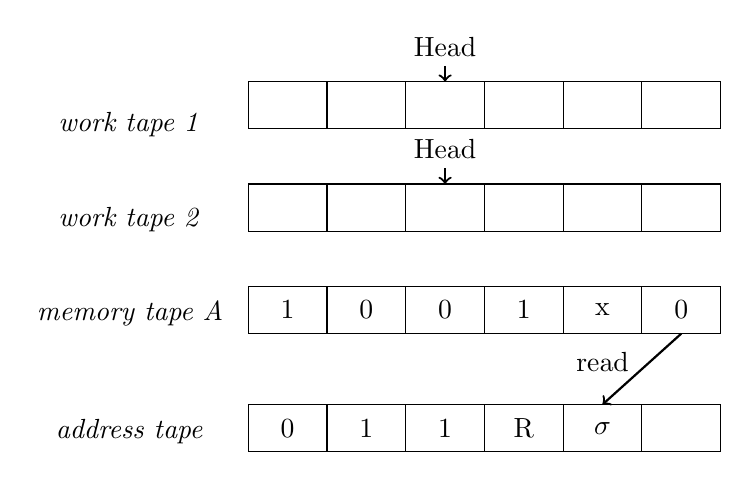
\begin{tikzpicture}
    \def\n{6}
    \def\cellwidth{1}
    \def\cellheight{0.6}
  
    \draw (0,2.6) rectangle (\n*\cellwidth, \cellheight+2.6);
    \foreach \i in {1,...,\n} {
      \draw (\i*\cellwidth,2.6) -- (\i*\cellwidth,\cellheight+2.6);
    }

    \node[above] at (\cellwidth*2.5, \cellheight+2.8) {Head};
    \draw[->,thick] (\cellwidth*2.5,\cellheight+2.8) -- (\cellwidth*2.5,\cellheight+2.6);

    \node at (-1.5,2.65) {\textit{work tape 1}};

\draw (0,1.3) rectangle (\n*\cellwidth, \cellheight+1.3);
\foreach \i in {1,...,\n} {
    \draw (\i*\cellwidth,1.3) -- (\i*\cellwidth,\cellheight+1.3);
}

\node[above] at (\cellwidth*2.5, \cellheight+1.5) {Head};
\draw[->,thick] (\cellwidth*2.5,\cellheight+1.5) -- (\cellwidth*2.5,\cellheight+1.3);

\node at (-1.5,1.45) {\textit{work tape 2}};
  
    \draw (0,0) rectangle (\n*\cellwidth, \cellheight);
    \foreach \i in {1,...,\n} {
      \draw (\i*\cellwidth,0) -- (\i*\cellwidth,\cellheight);
    }

    \foreach \i/\content in {1/1, 2/0, 3/0, 4/1, 5/x, 6/0} {
          \node at (\i*\cellwidth-\cellwidth/2, \cellheight/2) {\content};
        }

    \node at (-1.5,0.25) {\textit{memory tape A}};
    
    \draw (0,-1.5) rectangle (\n*\cellwidth, \cellheight-1.5);
    \foreach \i in {1,...,\n} {
      \draw (\i*\cellwidth,-1.5) -- (\i*\cellwidth,\cellheight-1.5);
    }
    
    \foreach \i/\content in {1/0, 2/1, 3/1, 4/R, 5/$\sigma$} {
          \node at (\i*\cellwidth-\cellwidth/2, \cellheight/2-1.5) {\content};
        }

    \node at (-1.5,-1.25) {\textit{address tape}};

    \node[above] at (\cellwidth*4.5, \cellheight-1.2) {read};
    \draw[->,thick] (\cellwidth*5.5,\cellheight-0.6) -- (\cellwidth*4.5,\cellheight-1.5);


  \end{tikzpicture}


\newpage
\begin{lemma}
    \textit{Let $L\subseteq\{0,1\}^*$. If L is decidable by an RAM Turing Machinein time T(n), then it is decidable by a multi-tape Turing Machine in time $O(T(n)^3)$. Moreover, if the length of the address is O(1), then L is decidable by a multi-tape Turing Machine in $O(T(n)^2)$}

    \begin{proof}
        \textit{Use an extra work tape as memory that contains pairs $(i,A[i])$, where i is an integer in binary, $A[i]\in\varGamma$, for all memory addresses that have been referred to.}

        \textit{To simulate one step of M, if M is in an access state, the new multi-tape Turing Machine M' will:}

        \begin{enumerate}
            \item scans tape A to find an address that matches i in the address tape
            \item if i does not exist, add a new pair $(i,A[i])$
            \item read or write $A[i]$ accordingly
        \end{enumerate}

        \textit{1,2,3 take $O(T(n)^2)+O(T(n))+O(T(n)) = O(T(n)^2)$}

        \textit{In total, M' runs in time $T(n)*O(T(n)) = O(T(n)^3)$}

        \textit{If address length is $O(1)$, then $\#pairs\leq T(n)$, length of each pair is $O(1)$,1,2,3 take O(T(n)) steps to simulate}
    \end{proof}

    \begin{remark}
        \textit{Ignoring polynomial factors, all Turing Machine variants are equivalent.}
    \end{remark}

    \textit{$\underbrace{C++}_{T(n)} \rightarrow \underbrace{Assembly Language}_{O(T(n))}\rightarrow \underbrace{RAM TM}_{O(T(n))} \rightarrow \underbrace{multitape TM}_{O(T(n^3))(\textcolor{red}{O(T(n^2))})} \rightarrow \underbrace{single-tape TM}_{O(T(n^6))(\textcolor{red}{O(T(n^4))})}$}

\end{lemma}

\begin{defn}
    \textit{Let $T: \N\rightarrow\N$, language $L\subseteq \{0,1\}^*$ is in \textbf{DTIME}(T(N)) iff there exists a multi-tape Turing Machine M that decides L in time O(T(n))}
\end{defn}

\begin{defn}
    $P = \bigcup_{c\geq1}DTIME(n^c)$
\end{defn}
\ifx\allfiles\undefined
\end{document}
\fi